%% Introduction


\section{Methods}
An overview of the physical components in the setup is shown in \autoref{fig:SystemOverview}.
\begin{figure}[H]
	\centering
	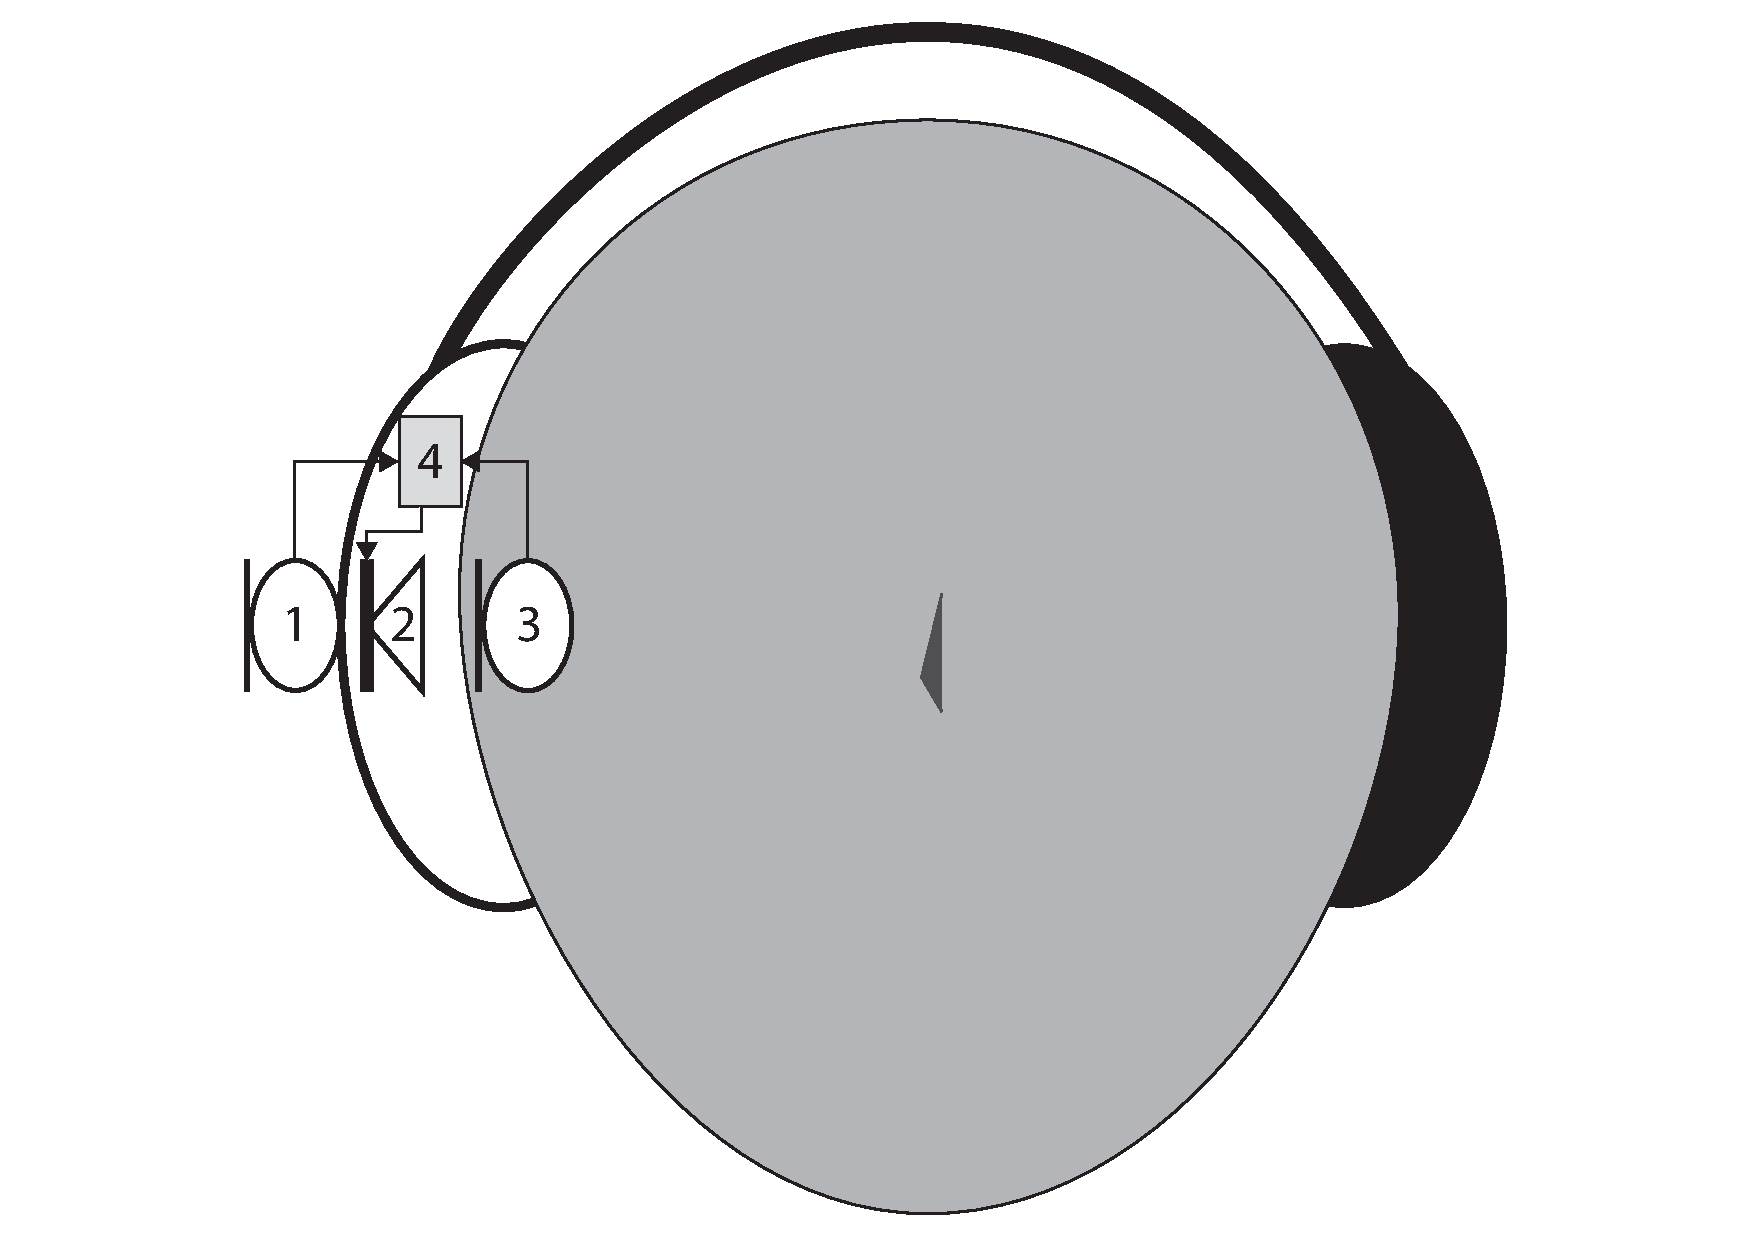
\includegraphics[width=1\columnwidth]{figures/ArticleIllustrations/SystemOverview}
	\caption{System Overview}
	\label{fig:SystemOverview}
\end{figure}
\autoref{fig:SystemOverview} is showing a head fitted with an ANC headphone using a reference microphone (1), a headphone loudspeaker (2), an error microphone (3) and a DSP (4).  

\subsection*{Feedforward ANC using FXLMS}

\begin{itemize}
\item BDD and explanation
\item FXLMS explanation + equation
\item Angle incidence 
\end{itemize}

The adaptive feedforward ANC system is shown on \autoref{fig:ANCFeedforward}
\begin{figure}[H]
	\centering
	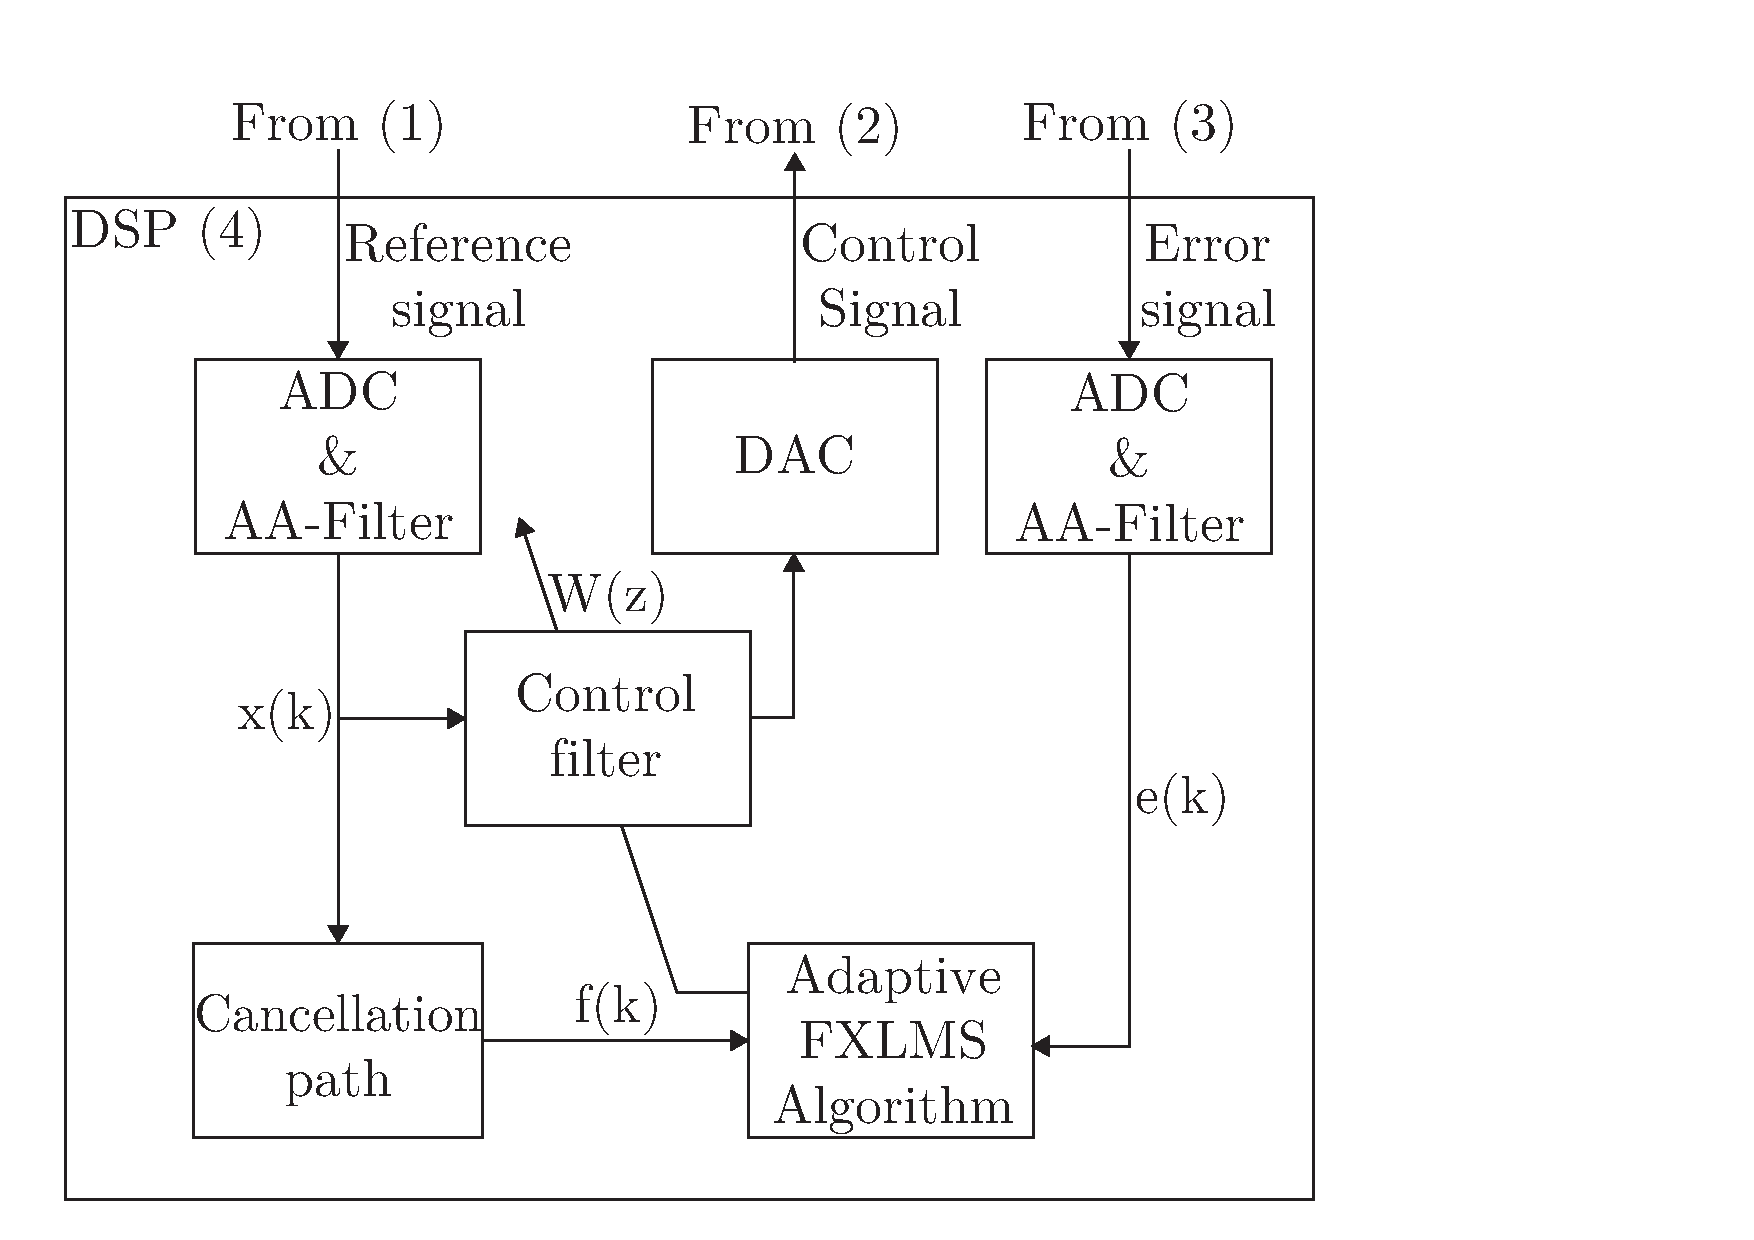
\includegraphics[width=1\columnwidth]{figures/ArticleIllustrations/ANCFeedForward}
	\caption{Adaptive feedforward ANC system}
	\label{fig:ANCFeedforward}
\end{figure}
\autoref{fig:ANCFeedforward} is showing an expanded version of the DSP block from \autoref{fig:SystemOverview}. This consists of converters, a control filter which is a FIR filter with coefficients adapted by the FXLMS algorithm. 

\textbf{Control Filter} is the filter representing the transfer function from the reference microphone to the headphone loudspeaker. The filter is initialized with the first 256 samples from the impulse response of the transfer function found by measurements \autoref{sec:AngleOfIncidence}.  

\textbf{FXLMS} is the optimization algorithm which updates the control filter coefficients using the FXLMS shown in \autoref{eq:FXLMS}. 

\begin{equation}\label{eq:FXLMS}
w_j(k+1) = w_j(k) - 2\mu e(k)f(k-j)
\end{equation}
Where:
\begin{description}
	\item[\text{$w(k)$}] is the weight coefficients of the control filter written as  $w(k)=[w_(k),w_1(k) \cdots w_{L-1}(k)]^T$
	\item[\text{$\mu$}] is the convergence factor
	\item[\text{$e(k)$}] is the error 
	\item[\text{$f(k)$}] is the reference convovled with the CP
\end{description}

\textbf{Cancellation Path} (CP) is the transfer function from the headphone loudspeaker to the error microphone. In the litterature \cite{Hansen} the CP is adaptively adjusted but it is assumed constant in this setup because the headphone is fixed.     



\subsection*{Linear Prediction}